Утилитарность может быть ординальна и абсолютна.

\textit{Определение:} \textbf{Функция утилитарности} это концепция, разработанная в области экономики и используемая в теории принятия решений.
Она описывает способность индивида оценивать полезность или степень удовлетворения от различных вариантов действий или состояний.

Происхождение функции утилитарности связано с развитием философской и экономической мысли. Одним из основоположников утилитаризма является Джереми Бентам. 
В XVIII веке и была разработана теория, согласно которой целью действий является максимизация утилиты --- суммарной пользы или счастья для всех членов общества.

\textit{Определение:} \textbf{Равновесие по Нэшу} --- состояние, в котором ни один игрок не может получить дополнительную выгоду от своих измененных действий, если другие игроки продолжают свои стратегии.

Классическим примером является дилемма заключенного.

\begin{figure}[h]
    \centering
    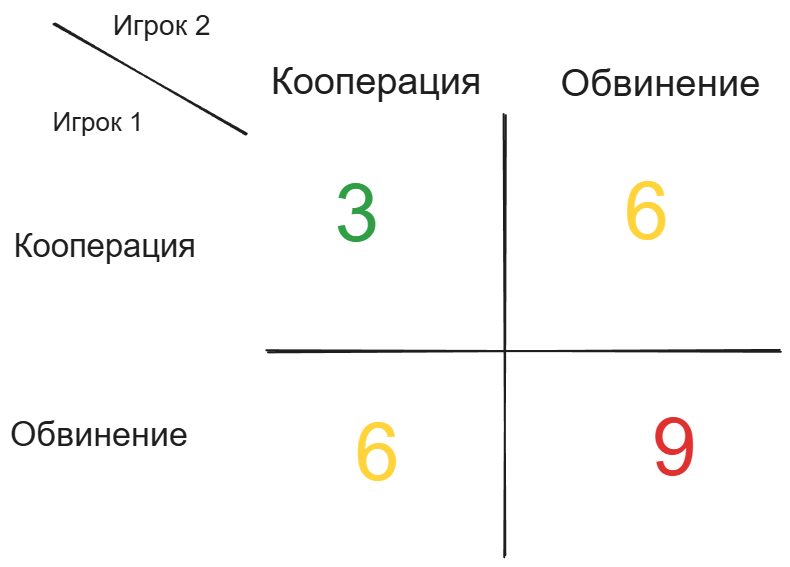
\includegraphics[width=0.5\textwidth]{assets/pedagogic/social/dilemma.excalidraw.png}
    \caption{Дилемма заключенного.}
    \label{dilem}
\end{figure}

Ординальная и абсолютная функции утилитарности представляют собой два различных подхода к измерению удовлетворения или полезности. 
В ординальном подходе утилитарное значение альтернатив оценивается лишь относительно других альтернатив, без установления конкретных метрик. 
Это позволяет определить порядок предпочтений между различными альтернативами, но не предоставляет количественной информации о различии в уровне удовлетворения. 
С другой стороны, в абсолютном подходе утилитарное значение измеряется в конкретных единицах, что позволяет проводить количественные сравнения между 
альтернативами и оценивать уровень удовлетворения более точно.

